% Set the author and title of the compiled pdf
\hypersetup{
  pdftitle = {\Title},
  pdfauthor = {\Author}
}

% Lecture 1

\section{The need for parallelism}

Even though we've been unable to increase the clock speed of processors since
around 2005, we have seen the `power' of processors roughly double every 18-24
months since then in line with Moore's Law\footnote{An observation that the
number of transistors in processor chips doubles approximately every two years.}.
The reason why, is that we have been able to increase the amount of transistors
in chips (due to the feature size decreasing), and use the extra ones to provide
more processing cores, which are able to process data in parallel. The degree of
parallelism is increasing as time progresses.

In an ideal world providing a greater degree of parallelism would merely entail
chip designers copy and pasting multiple processor cores onto the silicon, and
programmers getting linear performance increases. In practice, there are lots of
architectural issues (such as how processors are connected and how they're
organised) as well as software issues (how do we make our app run on multiple
cores).

As transistors are becoming smaller, we can also make them switch faster. The
switching speed is determined by $R*C$, where $R$ is the resistance and $C$ is
the capacitance. When we reduce the area of the transistor, $C$ decreases, so in
doing so, we make the circuit able to compute faster.

This was fine until 2005, at which point we started to see three problems which
stopped transistors from becoming smaller and faster:

\begin{description}
  \item \textbf{Interconnect capacitance}: the capacitance between neighbouring
  wires).
  \item \textbf{Power density}: As the power density increased, cooling became
  a serious problem; each transistor produces heat as it switches and the number
  of transistors per unit area dictates how much heat is produced.
  \item \textbf{Impurities}: As we approach the theoretical limit of one atom
  per transistor, any impurity in the silicon becomes a major issue.
\end{description}

We have tried using extra transistors to build more complex single core
processors (using Instruction Level Parallelism (ILP)) and by adding bigger
caches so that they exhibit lower miss rates, however both of these techniques
suffer from diminishing returns. Control statements such as \texttt{branches}
make us have to periodically throw away all the partially completed instructions
in a pipeline, and caches already have hit-rate percentages in the high $90$'s.

Though we might be able to increase the number of cores on a chip, how does a
programmer utilise this extra power? It is relatively easy for an operating
system to schedule programs so that they can run on different cores and
therefore have true multi-tasking (process level parallelism), but what if we
want to make one program run faster by running it over many cores?

\subsection{ILP vs TLP}

Instruction Level Parallelism and Thread Level Parallelism are two different
approaches to utilising parallel hardware, and both can be used at the same
time.

In ILP, the processor is able to execute instructions out of order and in
parallel, meaning that fewer clock cycles are needed to execute the same number
of instructions. This form of parallelism is very limited, and can only be used
in certain situations. Vector parallelism is similar, and lets you do things
like do four 8-bit additions in one instruction (by splitting a 32-bit word into
four 8-bit parts). In both cases, the end result of the execution is the same as
if all the instructions were executed in order.

In TLP, a program can be composed of separate threads, each being its own
sequence of instructions. Many threads can be executing in parallel and since
their instructions are independent of each other, can be interleaved on the
processor (or run on multiple cores). If it often desirable for the output of
threaded programs to be deterministic, i.e. for all possible sequences of
execution, the output must be the same.

TLP is far more general purpose than ILP (and much more so than vector
parallelism, which is only really useful in simple operations like array
addition). While ILP is applied automatically to the instruction stream issued
to the CPU\footnote{Either the compiler can make use of ILP (e.g. instruction
reordering at compile time), or the CPU can do it automatically using a
technique such as scoreboarding.}, whereas TLP relies on the programmer finding
a way to express an algorithm in a parallel manner; something that is not always
achievable for all programs.

% Lecture 2

\subsection{Data and instruction parallelism}

Flynn~\cite{flynn1972some} classified parallelism as \textbf{instruction stream}
and \textbf{data stream} parallelism, both of which can come into effect at the
same time.

Data parallelism is when the same computation can be carried out on multiple
elements of some dataset, usually an array. Vector parallelism is an example of
this. Only certain problems are amenable to data parallelism and can be sped up
in this manner, but doing so is often very easy\footnote{E.g. vector addition
can be easily parallelised by splitting the vector up into $n$ chunks and
assigning each one to a thread, where you have $n$ threads.}.

Instruction parallelism is when multiple instructions can be executed in
parallel (with no side effects that cause problems to each other), this is often
implemented automatically.

Flynn gave different combinations of these types of parallelism have different
names:

\begin{description}
  \item \textbf{SISD}: Single Instruction Single Data is like a normal program.
  A serial sequence of executions working on a stream of data, one word at a
  time.
  \item \textbf{MIMD}: Multiple Instruction Multiple Data is the most parallel
  one, where there are multiple instruction streams and they can all operate on 
  their own independent stream of data. This is what happens on most modern
  computer chips, where the operating system will schedule processes on
  different cores at the same time.
  \item \textbf{SIMD}: Single Instruction Multiple Data is stuff like when you 
  use instructions like \texttt{ADD8} to process multiple data elements at once 
  with the same instruction, or a GPU\footnote{GPU's often have upwards of
  hundreds or even thousands of processing cores, and in order to manage the
  complexity of assigning work to these cores, will use a combination of SIMD
  and SPMD techniques. The same program usually runs on each core, but groups of
  cores execute in lock-step on the same data.} processing lots of pixels at
  once with the same filter. If it's not a vector instruction, then it's one or
  more processors working in lockstep to process elements of an array or
  something.
  \item \textbf{SPMD}: Single Program Multiple Data is a generalisation of SIMD,
  where different processors execute the same code but don't need to be in 
  lockstep. This is most often how parallel programs are written for CPU's.
\end{description}

For any given problem, the complexity of parallelising it is proportional to how
irregular the parallelism is, and how much data sharing there is between threads
of execution (particularly if the threads are writing to the shared data).

\subsection{Connecting processors}

In order to make them work in parallel, multiple cores of a processor need to be
connected to each other, and to memory. There are lots of different ways to do
this, and the best way depends on the use case.

\begin{description}
  \item The processors can be laid out in a grid. In this case, each processor
  can communicate with its neighbours, and memory is usually private to each 
  core. In order for cores to access memory in other cores, they must send 
  messages through the grid.
  \item A Torus is a variation of the grid, where each edge is linked to the 
  opposite edge. This makes a doughnut shape (in a logical, not physical sense)
  and means that fewer steps are needed to communicate between cores.
  \item A bus can be used to connect multiple cores. The memory is usually
  situated on the bus, and all cores have access to it (though they may also
  have their own memory instead). Time slicing is used to give equal access to 
  the bus, but can make the bus become a processing bottleneck. All memory
  accesses have equal access time so long as there isn't too much contention.
\end{description}

There are, of course, more types of interconnects. Crossbars are where each node
is connected to each other node (which has a complexity of $n(n-1)$), but the
best ones are usually tree structures or hierarchical busses where the
complexity is logarithmic ($n log(n)$).

\subsection{Shared and distributed memory}

Shared memory is accessible from all of the cores and every part of the
computation, while distributed memory is spread out in different components, and
is usually only accessible by the component that owns it. We are considering
systems that are either one of these, or the other. Either one of these can
emulate the other from a software point of view; it is fairly easy to provide
abstraction layers that make a distributed memory behave like a shared one, or
impose restrictions on shared memory so that parts are unavailable to certain
components. Imposing a foreign memory layout onto the hardware comes at a
performance penalty.

More explicitly, \textbf{data sharing} is when a program with shared memory
space facilitates inter-thread communication by having threads read and write to
the shared memory. \textbf{Message passing} is when separate parts of the
program communicate by sharing messages (e.g. using a socket).

Most supercomputers use distributed memory, since its easier to build, provides
a higher total communication bandwidth and is more suited to many data-parallel
problems. However, programs using data sharing (shared memory) are widely seen
to be easier to code than programs using message passing (distributed memory),
so there is an overhead involved with distributed memory; unfortunately, most
`normal' computing problems are irregular and dynamic.

% Lecture 3

\section{Using threads}

A thread is a flow of control executing a program, and a process can consist of
one or more threads. Each thread inside a process has access to the same
address space, and most programming languages provide some method of using
threads.

Now, go and look up Java threads
(\url{https://docs.oracle.com/javase/tutorial/essential/concurrency/}) and C's
pThreads (\url{https://computing.llnl.gov/tutorials/pthreads/}).

The easiest form of parallelism to find and exploit using threads is data
parallelism. This is where computation is divided into roughly equal chunks,
where hopefully, each chunk is independent of the next.

An example of this is multiplying two $n\times n$ matrices. We could use $n^2$
threads, each computing one element (remember the area of the output matrix is
going to be $n^2$), or we could use $n$ threads and have each thread compute a
whole row or column. If we didn't have that many threads (or perhaps making more
threads is inefficient), then we could make $p$ threads and have each one
compute $q$ columns or rows, where $p\times q = n$.

In Fortran, \texttt{DOALL} statements let us execute the body of a loop in
parallel.

There are two types of parallelism:

\begin{description}
  \item \textbf{Implicit:} This is when the system works out how the parallelise
  something for itself. This is particularly relevant to functional languages,
  since many operations (map, reduce etc) are inherently parallelisable.
  \item \textbf{Explicit:} Here, the programmer must have a mental model of the
  parallelism in his or her head, and specifies exactly what should be done.
\end{description}

A lot of the time, parallel programs are made in a way that blends the two (so
you might not have to specify everything explicitly, but you have to give hints
to the system as to what should be parallelised and how). An example of this is
the \texttt{DOALL} statement mentioned above.

In an ideal world, we would have computers that would automatically parallelise
programs. However, since dependency analysis is hard to do, this approach is
limited. Computers do automatic parallelisation to an extent (e.g. instruction
reordering), but must be $100\%$ sure that an operation is safe to parallelise,
and the results will be correct.

% Lecture 4

\section{Caches in shared memory multiprocessors}

Obviously caches are vital to the efficient functioning of processors. Without
them, every memory access would cause the CPU to wait around 200 cycles, and so
having a cache is vital to having the CPU run at close to full speed.

However, caches don't just fix the problem; we need to work out how to populate
them, and keep the data in them correct. Data that we write to a cache must
eventually be written back to memory, and new memory locations need to be loaded
into the cache when they're required by the CPU.

We solved these problems in \texttt{COMP25111}, however, more problems arise
when you consider a multi-core processor. In most multi-core processors, each
core has its own cache, and since each cache can potentially hold its own copy
of the same memory location, we need to make sure that they agree with each
other about the values of these locations. This is the \textbf{cache coherence
problem.}

An easy solution to this would be to require that every write would go through
to memory straight away, and the other cache(s) in other cores would load the
value. This is obviously slow though and there may be bus bandwidth problems.
Furthermore, we'd only be getting a benefit from cache-reads, which defeats
(half of) the object of the cache!

We can overcome this by making the caches talk to each other. When a new value
is written to one cache, the others should invalidate their own cache lines
containing this value. This means a write to a cache doesn't need to go straight
through to memory, but just flips a bit inside the other caches.

However, when we introduce more state to our caches (such as invalidated cache
lines) we also increase the complexity, and need a model to make sure things
don't go wrong. Each cache line can be in three states:

\begin{description}
  \item Invalid; There might be an address math on this line, but the data is 
  not valid any more. It needs to be fetched from memory again.
  \item Dirty; The cache line is valid, and has been update in the cache since 
  it was loaded from memory. It must be written to memory at some point in the 
  future.
  \item Valid; The cache line matches what's currently in memory.
\end{description}

In order to let caches know what other core's caches are doing, we have them do
\textbf{bus snooping}. This involves having hardware watch each core's cache and
modify the cache independently of the core so that the flags on the cache lines
are correct.

Given two cores, the following states are valid and invalid (note that
some states are symmetrical):

\begin{center}
  \begin{tabular}{c|c c c}
      & V & D & I\\ \hline
    V & T & F & T\\
    D & F & F & T\\
    I & T & T & T
  \end{tabular}
\end{center}

Notice how the table is a mirror image of itself. We can't have two dirty
states, since then we won't know which we should write to memory, and we can't
have a dirty and valid state (since then, by definition, the valid state is not
valid).

We can analyse the state changes resulting from cores memory activity
by considering three aspects; accesses to memory, messages that need
to be sent between caches and the state changes that result.

\begin{description}
  \item \textbf{Transitions from \{D,I\}}:\\ Reading on the dirty core
  does nothing since a dirty value is always up-to-date, and writing
  to the dirty core will maintain its dirty status.

  If core two reads, then it gets the value from the first core and
  turns to valid. However, the state \{D,V\} is not allowed (since
  then consistency would be violated), so the first core writes its
  cache line to memory and the resulting state is \{V,V\}.

  If core two writes, then its state goes to D. However, there can't
  be two dirty cores, core two invalidates core one (this value is
  written back to memory) leaving the state in \{I,D\}.

  \item \textbf{Transitions from \{I,I\}}:\\ Reading from either core
  will make that core read the value from memory, which puts the
  reading core into a V state; \{V,I\} or \{I,V\}.

  Likewise, writing from either core results in that core going to the
  dirty state; \{D,I\} or \{I,D\}. Note that the newly dirty core will
  broadcast an invalidate message since it does not know the state of
  the other core.

  \item \textbf{Transitions from \{V,I\}}:\\ Reading from core one
  will do nothing, since the cache is valid, and reading from core two
  will request the value from the first core, leading to \{V,V\}.

  When core one writes, then it goes into the dirty state and sends an
  invalidate message to the other core (which does nothing); \{D,I\}.

  When core two writes, then it goes into the dirty state, but its
  invalidate message will cause the first core to be invalidated (no
  writeback is needed here since the line was only valid, not
  dirty); \{I,D\}.

  \item \textbf{Transitions from \{V,V\}}:\\ Reading from any valid
  state keeps the state valid and causes no invalidations.

  Writing to any of the cores will set that core to dirty and send an
  invalidate to the other core; \{D,I\} or \{I,D\}.
\end{description}

There are two types of messages between cores; read requests for a cache line
(one core hopes that another core's cache has the cache line so that it doesn't
have to go to memory), and invalidate messages.

We can easily extend the protocol we've described beyond two cores; any core
with a valid value can respond to read requests (the bus will decide who
`wins'), and invalidate requests work as normal, invalidating the cache line on
all cores.

The only extra requirement is that invalidation must happen in one cycle, since
we want all cores to have the same view of memory, and if one core receives the
invalidation message after another, there will be a period of time where their
views of memory will be inconsistent. This gets harder as we increase the number
of cores; the bus gets longer and so slows down (signals take longer to
propagate, and the clock will have to be reduced).

The impact from this is that the consistency protocol is the biggest limitation
when trying to add more cores to a processor. The protocol we have described is
called the \texttt{MSI protocol} (modified, shared, invalid).

% Lecture 5

\subsection{Other cache coherence protocols}

In the previous cache coherence protocols we have discussed, we came across
situations where there was unnecessary bus usage (e.g. when one core writes to
its cache and makes a cache line dirty, other cores would write their copies
back to memory, even though that value would never be used since there was a
newer dirty version).

However, the bus is a \textit{critical shared resource}, and we certainly don't
want to waste bandwidth on messages that have no effect. We can distinguish
between two cases of writing to a cache:

\begin{itemize}
  \item When the cache holds the only copy of a value, and it's not dirty (if it
  was dirty, we'd just update it).
  \item When the cache holds a copy of the value, but there are other copies in
  other caches.
\end{itemize}

It is only the first case where we don't need to send an invalidate message, but
this is nevertheless a common case. In most multithreaded programs, only a
minority of memory locations are shared between threads (and a smaller minority
are both read and written to by multiple threads), so the majority of memory
locations are unshared. If we split the `V' (valid) state into two more states,
we can account for this case:

\begin{itemize}
  \item \textbf{E} - Exclusive to one cache
  \item \textbf{S} - Shared between multiple caches
\end{itemize}

This gives us the \texttt{MESI} protocol (as opposed to the \texttt{MSI}
protocol). This is easy to implement on top of the \texttt{MSI} protocol; simply
set the state to E if the value was read from memory, and to S if it was read
from another cache.

Though minor changes in the protocol are required, the only inconsistency is
that if all E/S lines are evicted from other caches except one S line, then the
S line is now exclusive (even though it is marked as S). This isn't a problem in
practice, since it doesn't happen often, and since it's hard to detect, it's
just ignored.

The \texttt{MOSEI} protocol is a further optimisation, where the M state is
split into:

\begin{itemize}
  \item \textbf{M} - Modified; the cache contains a copy which differs from 
  memory, and no other caches contain a copy.
  \item \textbf{O} - Owned; the cache contains a copy which differs from the one 
  in memory, and some other caches also contains a copy, but those are in state 
  S and have the same value as the owner.
\end{itemize}

With the additional O state, we can share the latest value and don't have to
write it back to memory straight away. Only when a cache line in the O or M
states is evicted, will any writing to memory be done.

\subsection{Directory based coherence}

So far, we've looked at methods for letting multiple cores communicate over a
single bus, and have assumed that bus communication happens instantaneously.
However, as the number of cores increases, the bus capacitance increases and you
have to slow it down. This limit is at around 32 cores.

A directory based coherence method is an attempt to make everything less
directly connected to get around this limitation. A centralised directory is
created that holds information about each cache line (which contains multiple
words) in memory.

For each cache line, the directory contains a bit map for which core has a copy,
and whether that copy is dirty, which is another bit map (though only one bit is
true). Each cache has its own valid and dirty bits, which are used to dictate
whether to write back to memory or not. If a core whats to make a memory access,
we have the following cases:

\begin{description}
  \item \textbf{Read hit in local cache}:\\
    Just read the local value!
  \item \textbf{Read miss in the local cache}:\\
    Ask the directory:
    \begin{description}
      \item \textbf{Directory dirty bit is false}:\\
        Read the data from main memory into the cache, set the directory
        presence and local valid bit for that core.
      \item \textbf{Directory dirty bit is true}:\\
        Cause the owner to write back the value to memory, which is also sent to
        the cache that was asking. The directory dirty bit is cleared, but the
        directory presence bits are set, as is the local valid bit.
    \end{description}
  \item \textbf{Write miss in the local cache}:\\
    \begin{itemize}
      \item Set the local cache to dirty.
      \item Depending on the directory dirty bit:
      \begin{description}
        \item \textbf{It's false}:\\
          Invalidate any cores that are valid for this cache line, set the
          present bit for that core and set the dirty bit for the directory.
        \item \textbf{It's true}:\\
          Send a message to the core marked as O (owner) to write back (note,
          this can be optimised out). Clear the owner's present bit, and set
          if for the writing core. Leave the dirty bit set.
      \end{description}
    \end{itemize}
  \item \textbf{Write hit in local cache}:\\
    \begin{itemize}
      \item If the local dirty bit is set, just update the value,
      \item Otherwise, update the local cache and dirty bit then:
      \begin{description}
        \item \textbf{If the directory bit is not dirty}:\\
          Invalidate any cores with the cache line present, then clear the
          present bits.. After that, set the present bit for the writing core
          and set the directory dirty bit to true.
        \item \textbf{If the directory dirty bit is set}:
          Send a message to the owner to update core memory (again, this can
          be optimised out), clear the owner's present bit and set the
          writing cache's present bit. Keep the directory bit set.
      \end{description}
    \end{itemize}
\end{description}

In this architecture, the directory becomes the bottleneck. To avoid this, we
can distribute the directory between different caches, and make each part
responsible for part of the address space. Sometimes in multi-processor systems,
the memory is not all in one place and is spread over multiple chips.

Since chips with a directory based protocol are often heavily networked (inside
the chip) in order to connect all the sub-components, messages can take variable
amounts of time to send, requiring handshake protocols. This means that the CPU
can sometimes waste a significant number of cycles waiting for responses from
messages.

% Lecture 6

\section{Barriers and locks}

\subsection{Barrier}

The idea of a barrier is that a number of threads should all meet up at the same
point. When all threads reach the point, they can continue, but until then, they
all wait. It's natural when threads are used to implement data parallelism.

Barriers are often used when there are data dependence (we need to wait for the
whole answer before continuing). Take a look at
\texttt{java.util.concurrent.CyclicBarrier}.

\subsection{Locks}

Any object can be locked in Java by using as the target of a
\texttt{synchronised} block, or calling an instance method that is declared as
being \texttt{synchronised}. Only one thread can lock an object at any given
time, and other threads must wait to acquire the lock, or the lock holder
executes \texttt{wait}.

We want to lock objects so that we can achieve `correctness'. If two code blocks
take a lock on the same object, one should complete before the other starts,
which means two threads won't be mutating the same object at the same time, and
the normal meaning of the code blocks is preserved.

% TODO: Implement a bounded buffer like in the notes

\textbf{Sequential Consistency} is when:
\marginpar{This is a common interpretation of what it means to be `correct',
but not the only one.}

\begin{itemize}
  \item Method calls should appear to happen one at a time in sequential order.
  \item Method calls should appear to take effect in the order a thread performs
  them.
\end{itemize}

Deadlocks can occur in cases where code tries to acquire more than one lock.
`Lost WakeUp' can happen if one thread sends a \texttt{notify} message that is
not properly received by other threads, one way to avoid this is by using
\texttt{notifyAll} instead of \texttt{notify} in Java.

The \textbf{granularity} of the lock depends on how big the chunk of code that
depends on a lock is. If the chunk is large, then it's coarse grained and the
parallelism is more limited, and if its too small, then its fine grained, and
you may spend too much time obtaining and releasing locks.

Java also has \texttt{java.util.concurrency.locks.Lock} for explicit locks,
since there are situations where the implicit object locking is not adequate. An
example of this is when doing `hand over hand' locking (e.g. lock one item,
obtain the next, lock the newly obtained one, unlock the first etc). This is
impossible using the implicit locks, since there is an implicit nesting structure
(e.g. a synchronised call is either inside a synchronised block or in a
synchronised method call, and you can only get out by exiting the whole block).

% Lecture 7 - Hardware support for synchronization

\section{Hardware support for synchronisation}

Most shared memory parallel Programming models require that the programmer
implements some sort of synchronisation logic in order to control how threads
access the shared memory. There are several different ways of doing this, all of
which are closely related. Hardware support is usually required for shared
memory multiprocessor systems.

\subsection{Binary semaphores}

A \textit{binary} semaphore is essentially a boolean indicating whether some
resource is free; (\texttt{1} $\rightarrow$ free, \textit{0} $\rightarrow$ in
use).

There are two atomic operations that can be done on a semaphore;
\texttt{wait(s)} and \texttt{signal(s)}. \texttt{wait} will block until
\texttt{s} is equal to $1$ (i.e. wait until it's free), then set \texttt{s} to
$0$. \texttt{signal} sets \texttt{s} to be equal to $1$. For example:

\begin{minipage}{0.5\textwidth}
\textbf{Thread \#1}
\begin{verbatim}
wait(S)
print "Thread 1 says 'Hi'"
signal(S)
\end{verbatim}
\end{minipage}
\begin{minipage}{0.5\textwidth}
\textbf{Thread \#2}
\begin{verbatim}
wait(S)
print "Thread 2 says 'Hi'"
signal(S)
\end{verbatim}
\end{minipage}

A \textbf{broken} implementation of \texttt{wait} could be:

\begin{verbatim}
  # Move the address of the semaphore into R2
  ADR   R2, semaphore

  ...

  wait:
        PUSH LR
        PUSH R1
  loop: LDR R1, R2
        CMP R1, #0
        BEQ loop
        STR #0, R2
        POP R1
        POP PC
\end{verbatim}

The reason why this wouldn't work, is that if another thread was to
change the value of the memory address pointed to by \texttt{R2} while
were were inside
\texttt{loop}, then we could get unpredictable results.

In order to prevent this from happening, we need to make sure
that \texttt{wait} is indivisible, which requires special hardware
instructions. Even then, if
\texttt{semaphore} was cached, then even indivisible waiting methods might get
confused, so we need coherence operations in the cache.

A simple solution (often implemented in older processors) is to
provide an instruction called \texttt{test and set}, which is
atomic. This takes a pointer as an argument, and tests if the memory
location is \texttt{0}. If it is, then the memory location is set
to \texttt{1}, and if its not, then the processors zero flag is
cleared. Now our wait function becomes:

\begin{verbatim}
  # Move the address of the semaphore into R2
  ADR   R2, semaphore

  ...

  wait:
        PUSH LR
        PUSH R1
  loop: TAS R2
        BNZ loop # loop while *R2 != 0
        POP R1
        POP PC
\end{verbatim}

Note that this is the logical opposite of how we defined the semaphore
before, but it doesn't matter. Furthermore, though it looks like we've
reduced the number of instructions, the \texttt{TAS} operation will be
slow since it must read and possibly write a value in memory, which
requires that memory location to be locked.

If \texttt{semaphore} is cached, (which is likely since its going to
be a shared memory location), then we're going to be using a lot of
bus bandwidth because the processor must lock the snoopy bus for
every \texttt{TAS} operation since it cannot let other cores write to
that memory location. If the value of the semaphore was $1$, then the
lock was wasted.

A simple solution is to sit in a loop reading the value of the
semaphore until it seems to be free, then use a \texttt{TAS} operation
to obtain the lock. If the \texttt{TAS} operation was successful, then
return to the calling code, and if it wasn't, then another thread must
have got there first and the current thread should continue looping:

\begin{verbatim}
  # Move the address of the semaphore into R2
  ADR   R2, semaphore

  ...

  wait:
        PUSH LR
        PUSH R1
  loop: LDR R1, R2
        CMP R1, #1
        BEQ loop
        TAS R2
        BNZ loop
        POP R1
        POP PC
\end{verbatim}

\subsection{Other synchronisation primitives}

There are other machine level primitives including \texttt{fetch and
add} (get a memory location, add one and write back),
and \texttt{compare and swap} (compare a memory location to a value
and exchange it for another value if it was as expected). These are
read-modify-write instructions and require the snoopy bus to be locked
while they execute.

The trouble with these operations, is that they are quite complicated
(i.e. like CISC instructions, not RISC instructions), and as a
consequence, they don't fit well with modern pipelined processors.

There are two instructions called `Load Linked' (\texttt{LDL Rx, Ry})
and `Store Conditional' (\texttt{STC Rx, Ry}) respectively that are
essentially atomic loads and stores.

\texttt{LDL Rx, Ry} loads the value of the address \texttt{R2}
into \texttt{R1} but also sets a special `load linked' flag on the
processor core executing the instruction. The address \texttt{R2} is
stored in a `locked address register' on that core.

\texttt{STC Rx, Ry} stores the value in \texttt{Rx} into the location
addressed by \texttt{Ry}, but it only works if the `load linked' flag
is set. The value of the load linked flag is returned in \texttt{R1}
(if the store was successful or not), and the load linked flag is
cleared.

The load linked flag is unset if another core writes to the address
that is stored by the load linked register (if an invalidate message
was received that matches the value in the register). This occurs when
a write has occurred to the shared variable, and hence whatever
operation we were working on with our core wouldn't be atomic.

Here is a correct implementation of the semaphore:

\begin{verbatim}
loop: LDL R1, R2 # Load link the address of R2 into R1
      CMP #0 R1  # See if the load link worked?
      BEQ loop   # If not, then try again
      MOV #0 R1  # Overwrite the register
      STC R1, R2 # Try and write it back to memory
      CMP #1 R1  # If R1 is set, it worked
      BNC loop   # Loop back if it didn't work
\end{verbatim}

This works because any other core writing to the address
in \texttt{R2} between lines $1-5$ will cause the load link flag to be
unset, causing the \texttt{STC} instruction to fail.

We have seen the Test and Set instruction, and the Load Linked/Store
Conditional instructions. These are both useful and can guarantee
atomicity, though LL/SC can guarantee atomicity of anything between
the two instructions, while TAS is only atomic within itself.

Implementing locks as we have above results in a \textbf{spin lock},
where the processor will sit and continually check to see if the
condition is such that it can proceed (also known as a busy wait or
spinning). It is more efficient (especially for power in things like
mobile phones) if the processor can switch off for this duration, or
switch to another thread. Other forms of locking enable this, though
the basic hardware support is similar or the same.

% Lecture 8 - Lock free datastructures

\section{Lock-free datastructures}

We have seen datastrucutres that employ locks, barriers and other
synchronisation primitives in order to serialise multithreaded access
to them, but instructions such as \texttt{compare and set} can be used
to make sure that updates to datastructures happen in a serial manner,
while removing the need for locks.

Let us take the example of an unbounded queue, implemented using a
linked list. A locking implementation might use two locks; one for
pushing and one for popping (though these locks must be aware of each
other when the queue is empty); implementation details are covered in
the lecture notes (but not here). Only one thread can push and one pop
from the queue at the same time, which obviously becomes a bottleneck
when multiple threads are accessing the queue.

With Java's \texttt{java.util.concurrent.atomic.AtomicReference}
and \texttt{compareAndSet} features, we can make the same
datastructure with no locks. Though there is still an overhead
associated with multiple threads accessing the queue, they are held in
busy-loop style constructs made from RMW\footnote{Read, Modify, Write}
instructions such as Compare and Set. Though an awareness of lock-free
datastructures is required for the course, understanding an
implementation is not.

% Lecture 9 - OpenMP & MPI

\section{OpenMP \& MPI}

OpenMP and MPI\footnote{Message Passing Interface} are two common ways
of parallelising programs, usually with C, C++ or Fortran.

\subsection{OpenMP}

OpenMP is a set of compiler directives and library functions that let
the programmer give hints to the compiler and OpenMP framework about
how to parallelise the program. OpenMP has a fork-join model of
threading, and tries to provide sequential equivalence\footnote{The
result of the program should be the same running in parallel as it
would be running on a single thread.} and incremental
parallelism\footnote{Incremental parallelism is where you write the
program as normal, and then gradually parallelise more and more of
it.}.

Parallelising with OpenMP is really quite easy, only one compiler
directive is needed to parallelise a code block, for example:

\begin{verbatim}
  int i = ...;
  #pragma omp parallel num_threads 3
  for (i = 0; i < n; i++) {
    loop_body;
  }
\end{verbatim}

As is usually the case with C/C++, and variables declared inside the
parallel block are private are scoped solely within the block, but
since the block is initialised on many threads, these variables are
private to each thread too. Variables declared before the parallel
block are shared. All code blocks parallelised with directives must
have a single start and end point, and an implicit thread barrier is
used at the end to ensure that all threads have finished before the
program moves on from the block.

\subsubsection{Worksharing}

\marginpar{N.b. If you have each thread returning a result (maybe
you're adding a number to a sum on each iteration), then you should
store these results in an array and then combine them (e.g. do the
summation) once the parallelised loop has finished. Writing to the
same memory locations in a parallel block will cause memory
consistency problems.}

Running a program with multiple threads is pointless if all the
threads do the same thing; instead, we want to split the total work as
evenly as possible between them. An easy way to do this is by
using \textit{loop splitting}, where a time consuming loop is
restructured to make each iteration independent of each other, and
then all the iterations are split between all of the available threads.

Many loops will have some kind of updating happen on each iteration of
the loop, such as an addition or finding the minimum of the results of
the iterations. Many of these updates are associative; i.e. they can
be applied in any order, and as such, OpenMP has directives to apply
them in a thread-safe manner (called a reduction clause). If we wanted
to sum an array we could do:

\begin{verbatim}
  int[] myArray = ...
  int sum = 0;
  #pragma omp parallel for private(x) reduction(+:sum)
  for (int i = 0; i < n; i++) {
    sum += myArray[i];
  }
\end{verbatim}

OpenMP has other synchronisation constructs too, such
as \texttt{flush} which ensures memory consistency between
threads, \texttt{critical} which indicates a critical
section, \texttt{barrier} which is an explicit barrier for the
threads, and more.

\subsubsection{Loop Scheduling}

Loop scheduling is deciding which iterations should be run on which
threads. For efficiency reasons such as maximising cache usage, it is
usually desirable to allocate iterations in chunks, however this can
be done at runtime (dynamically), or at compile time
(statically).

Static loop scheduling has three common methods:

\begin{itemize}
\item Block schedule is when the iterations are split into chunks of
approximately equal size.
\item A Cyclic schedule is when one iteration is given to threads in
turn until all the iterations are assigned.
\item A block-cyclic schedule is the same as a cyclic schedule, but
$n$ iterations are assigned to each thread each time. This is more
cache friendly.
\end{itemize}

\subsection{MPI}

MPI (message passing interface) can be used to program a wider variety of architectures than
OpenMP since it is able to distribute work between multiple computers
(distributed memory systems). Like OpenMP, it is a library for C,
Fortran and other programming languages.

MPI works by sending message between processes; each message is
identified by a triple \texttt{<send\_proc\_id, recv\_proc\_id,
tag>}. MPI has a concept of \textit{communicator contexts} which are
initialised to facilitate message passing between processes. The same
message tag can be used between different contexts, but only once
within a single context.

Perhaps the easiest to understand MPI commands are its blocking send
and receive commands\footnote{These are listed in the course notes
along with MPI examples, but I can't see much benefit to listing them
here too.}, but MPI also has barriers, broadcast, scatter, gather and
reduce constructs. As a result of having these more complex, higher
level commands, many programs don't use `send' and `reduce' very much.

MPI also supports asynchronous commands, which do not block the
sending/receiving thread, as well as persistent communication (i.e. the
same connection is kept open to send multiple messages in a stream
like fashion).

% Lecture 10 - Speculation

\section{Speculation}

Speculation is when a processor isn't sure whether an execution needs
to be executed (i.e. the result of a branch or conditional operation
isn't yet known), but since there are functional units free on the
processor, the result can be computed speculatively and discarded if
it is not needed. This assumes the `recovery' cost of a wrong decision
of what to speculatively execute isn't too high.

The only resource that is wasted by speculative execution is power,
since the resources would otherwise be idle.

Sometimes, it is advantageous to speculatively parallelise
programs. If we're not sure if a program can be safely parallelised,
we could parallelise it anyway, and see if the result is still valid
afterwards. Thread Level Speculation is a technique for doing this;
the idea is to divide single threaded code into separate treads, run
them in parallel and detect (with a view to resolving) any problems at
runtime.

As you will know if you took the Compilers course, you'll know that
loops can be trivially parallelised\footnote{Simply assign iterations
of the loop to different threads.} if there are no dependencies
between iterations of the loop. Simple dependencies can be recognised
and in some cases (usually when there is a nested loop, and the
dependency is in the inner loop), the code can be optimised so some
operations can be parallelised.

However, if the loop is complex (usually when we don't know the index
of an array access until runtime), then we could do loop based thread
level speculation.

If the index of the array $j$ we're accessing in the loop is less than
the iteration count $i$, then we use a value that we've already
computed. If the $j$ is greater than $i$, we must use the value that
was in the array before we started the computation. This is an issue
because if multiple threads are updating the same array (and they
could be updating any index in the array), then we will probably end
up corrupting memory.

Lets say we have the following loop:

\begin{verbatim}
for (int i = 0; i < N; i++) {
  A[i] = A[g(i)] + 1
}
\end{verbatim}

Here, we set the array value at $i$ to the value of the index
designated by the function $g$ plus one. In order to parallelise this,
we could have a single thread for each iteration, but only let the
first thread ($i=0$) update the original array. All the other threads
must maintain their own copies of the array.

Each thread then maintains a tag on each of its array indexes, which
can be in one of four states:

\begin{itemize}
\item Not accessed (N)
\item Modified (M)
\item Speculatively loaded (S)
\item Speculatively loaded and later modified (M)
\end{itemize}

This information is usually held in a separate datastructure from the
array itself which is visible to all threads. All threads write to
their own data and mark the data item as `M' (or `SM' if it was
already marked `S'). Any thread reads its own data if the state is not
`N' (i.e. untouched), otherwise it looks at the tag that the threads
`below it' (iteration wise) for a value that is not `N' (or until it
reaches 0) and then reads the value into its own copy of the array,
marking it `S'.

Any write can cause a conflict, and if a higher numbered thread has
the state of the written index as `S' or `SM' then they have
speculatively read a thread before it was ready. The most simple
solution to this is to abort all the threads above the offending
thread and restart them.

At some point, the data from all of the speculative threads must be
reconciled, which is done every time a thread completes, the thread
after it becomes non-speculative and writes its modified values back
to the main array. Eventually, all the threads will terminate and
commit their data.

\begin{figure}[H]
\centering
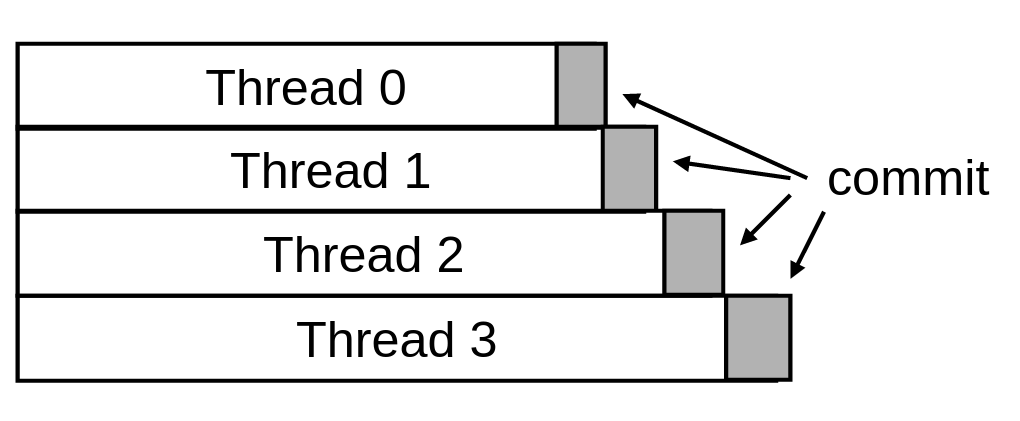
\includegraphics[width=0.7\textwidth]{diagrams/commit-diagram}
\caption{A visualisation of how the threads could run; each thread
must wait for the previous one to finish and for its data to become
non-speculative before it can itself commit its data and exit.}
\end{figure}

Of course, this all introduces an overhead on each memory access as
well as the overhead of running multiple threads, yet with the right
sort of programs, the speed up can be 2x faster on four cores or 3x
faster on 8 cores.

In theory, we could make hardware support for this by using the cache
for the speculative buffers. However since the cache size is very
limited, this would only work for small buffers, and/or small numbers
of threads. By modifying the cache protocols to make sure data is not
written to memory too early, and to use snooping buffers to detect
conflicts, this could be implemented efficiently.

\subsection{Procedure based TLS}

If we limited ourselves to parallelising only loops, then we would
only speed up a small portion of code. If we could parallelise
functions/procedures, then we could potentially gain a lot of
speed. This would work by executing the code serially, but splitting
the execution into two threads when there is a procedure call. It is
the \textbf{code after the procedure call} that is run in a new thread
(and the body of the procedure is run in the main thread), since then
it can be easily abandoned if required. Validation is typically done
at the end of the procedure call (to check if the threads had
conflicting memory accesses). If the validation passes, then the
speculative thread continues as the main thread.

\subsection{Sharing resources}

We can also use speculation to allow multiple threads to access a
resource. Classically, we would need to use a lock to make sure the
threads access the resource in a mutually exclusive manner, but much
of the time (e.g. writing to different parts of a file), the writes
would not conflict.

% Lecture 11 - Transactional Memory

\section{Transactional Memory}

Thread level Speculation (TLS) tries to guess if parallelism is
possible and valid without help from the programmer. Transactional
memory provides the programmer with transactions within a parallel
sharing context. This means that the memory implements ACID:

\begin{itemize}
\item Atomicity; all or nothing
\item Consistency; one valid state leads to another
\item Isolation; each transaction is isolated from all others 
\item Durability; once committed, the outcome is persistent
\end{itemize}

Only atomicity and isolation are relevant to TM.

Transactions are indivisible, so that a transaction executes either
completely, or not at all. While it is executing, none of the
transaction's changes are visible outside the transaction.

When it completes, the changes will all happen at the same time.

Essentially, you can use transactions where you would previously have
used locks:

\begin{verbatim}
  atomic {
    i += 2;
    j *= 5;
  }
\end{verbatim}

Locks are fine if you're only using one, but if there are multiple,
then the potential for deadlock is always there. Transactions do away
with the potential for deadlock, since they are composable (where
locks are not).

The format of a transaction is as follows:

\begin{itemize}
\item The transaction starts
\item Some shared variables are read
\item Some writes are made
\item The transaction tries to commit
\item This will succeed if there's nothing wrong...
\item ... or will abort if it cannot commit, and then the whole transaction must be repeated.
\end{itemize}

There are two reasons why the transaction may abort; either there has
been a read-write clash, or a write-write clash. These clashes cannot
be tolerated, since they would allow programs to get results that
would violate either atomicity or consistency.

To implement transactions, the the variables that have been read need
to be kept track of (the readset) and the variables that have been
written to need to be kept track of too (the writeset). These two set
are used to determine clashes with other transactions.

An application for TM is routing; we have a number of points in a 2D
plane that we want to make connections between, and the connections
cannot cross each other (e.g. on a Printed Circuit Board). We could
solve this by representing the plane as a 2D array of integers that
encodes what is in each cell, and then we can find the routes between
the connections in parallel so long as we avoid intersections.

Of course, avoiding intersections is the hard bit. The easy way it so
lock the array (and therefore get no parallelism), or we could lock
individual cells (i.e. have a thread find a route, lock the whole
route and then unlock the route when it's done), however this is hard
to correctly and without introducing a bottleneck.

With transactions, we can use one transaction for each required
track (and that's it). So long as there aren't too many tracks, then
the performance is good in parallel.

\subsection{Versioning}

If a transaction writes to a variables and reads the written value
later, then the updated value should be visible, not the original
one, yet if the transaction aborts, then the original
value needs to be preserved. We need some kind of versioning to
implement this:

\begin{description}
\item \textbf{Direct updating} (aka eager versioning) is when the transaction will
change the shared variable, but log the change privately. If the
transaction commits, then it will discard the log, but if it aborts,
then it will undo the writes present the log. This is efficient if
aborts are rare, and only works if the transaction clash detection is
bulletproof.
\item \textbf{Deferred updating} (aka lazy versioning) is the opposite of
direct updating, where a private version of the changes to the shared
variables is maintained, which can be thrown away on an abort. On a
commit, the thread would copy the privately held values in the log to
the shared variables. This is efficient if aborts are more common than
commits.
\end{description}

As mentioned, both of these methods rely on being able to detect
clashes. This is called \textit{validation} (or conflict detection),
and can, like updating, be done in a lazy or eager manner:

\begin{description}
\item \textbf{Lazy Validation}: This is done when the transaction is
about to commit. Here, we know the details of all of the reads and
writes that occurred in the transaction, so we can just detect
conflicts from these.
\item \textbf{Eager Validation}: Every write operation to a shared
variable in a transaction can cause other transactions to see if they
have clashed. We can then choose which transaction to abort or
possibly delay a transaction to let another finish first. We need to
make sure that we don't accidentally cause livelock here.
\end{description}

Unlike for updating, we can mix the two at the same time, using one
method for reads, and another for writes.

Other design options for transactions include strong and weak
isolation (allow access to shared variables only within transactions
or from anywhere), and enabling nesting transactions (transactions
within transactions), which is essential for composability.

\subsection{Hardware support}

There are implementations of transactional memory in Java and C (and
probably other languages), but when there is lots of sharing, the
performance isn't great. However, in situations where you really don't
want to use barriers and locks, this might be an acceptable trade off.

Implementing transactions in hardware could alleviate the performance
penalties, and all of the big processor developers (Intel, AMD, ARM)
are looking into it. The idea is that certain portions of the program
would be declared to be atomic, and all memory accesses in that
portion would be emulated using two sets; a \textit{readset} and
a \textit{writeset}. If another thread writes to something in the
readset, then abort the current transaction, and if the end of the
transaction is successfully reached, then commit the writeset to
memory.

The load-linked an store-conditional commands are essential a
transaction, since the readset is the single memory location being
read-modify-write accessed and bus snooping is used to detect if
changes were made to the register during the transaction (clearing the
load linked flag if so). The store-conditional operation `commits' the
transaction if no conflict was detected, and otherwise, a jump
instruction will be used to abort and restart.

In order to extrapolate the approach to multiple memory locations, we
can use the cache as a buffer to keep track of the readset and
writeset. This requires extra cache flags to indicate the data was
read or written inside an atomic block, a modified writeback behaviour
(only write back if the transaction commits), and an altered snooping
protocol.

The snooping protocol must be changed so that when a transactional
variable is written, the invalidate message is broadcast as usual, but
if another core receives an invalidate message that matches a location
in the readset, then it must invalidate the transaction. When the
transaction terminates, the writeset is flushed to main memory. This
latter stage may require synchronisation since the operation must be
atomic.

Obviously, if we're using the cache to store or readsets and
writesets, then the size of each is limited by the size of the
cache. Furthermore, we must make sure that cache entries that are part
of transactions are not evicted since otherwise the data will be lost
(since it cannot yet be written back to memory). Livelock can occur if
three or more transactions cause each other to abort in a cycle.j

Instead of using a cache-based implementation, we could use a snooping
bus (which doesn't handle large numbers of cores well) or do away with
cache coherence and make all accesses to memory transactional.

\subsubsection{Transactional Coherence and Consistency}

TCC is a simple protocol designed to implement hardware
transactions. Though it is simple, there are many possible
optimisations, but as of yet, no implementations.

The idea is to have a local cache for each core that stores the
readset (as well as other cached data), but the writes are stored in a
separate buffer (such as in RAM). Writes to shared data can only occur
in transactions, and are therefore locally buffered, meaning
invalidations are not broadcast. It is only when the transaction
completes that its writeset is written back to memory, and to do this,
the addresses of its writeset are broadcast to other cores (in a
single packet), and if other cores detect a conflict, the detecting
core should restart its transaction.

The main disadvantage of this is that there needs to be some central
lock to ensure that only one transaction is being committed at once,
though transactions that do not overlap can be committed concurrently.

The advantages of TCC are:

\begin{itemize}
\item Lazy conflict detection.
\item Livelock is impossible since one of the conflicting transactions always completes.
\item Inter-core synchronisation only occurs at commit time.
\item Instantaneous communication is not required.
\item Less communication between cores (in many cases), meaning more cores could be supported.
\end{itemize}

\subsubsection{Hybrid Transactional Memory}

The limited size caches and buffers are of limited size, so the
current best practice is to keep transactions as small as possible so
there is a high chance that they will by fulfilled entirely in
hardware (and a low probability of conflict), but overflow to software
if required.

% Lecture 12 - HW support for transactions

\subsection{Hardware support for Transactional Memory}

Since transactional memory could significantly simplify the
programming model, there is interest in a hardware implementation
rather than emulation support with software (which becomes non-optimal
for programs that do significant amounts of data sharing). Multiple
hardware manufacturers are working on hardware TM.

The idea is to declare sections of code as atomic, probably using a
special instruction, and then keep note of all the addresses loaded
from (the readset) and buffer all the writes (the writeset) for the
duration of the atomic section. If another thread writes to something
in the readset of our atomic section, then the transaction must be
aborted (simply get rid of the buffered writes) and restarted. If, on
the other hand, the transaction successfully completes with no
conflicts, then the writeset can be written back to memory
(committed).

In fact, load-linked and store-conditional instructions are
transactions, which is why they appear atomic. The readset is a single
variable being RMW accessed, and the address is stored in a
load-linked register. Bus snooping detects any writes to this address,
and the load-linked flag is cleared if a conflict is detected (which
causes the store-conditional operation to fail, and the program flow
to be redirected to try the transaction again).

However, unlike using load-linked registers, complex transactions
involve a significant number of variables to be read and written. We
can regard the CPU cache as a buffer to store both the readset and the
writeset. This requires the following:

\begin{itemize}
\item Adding extra tags to the cache entries to
indicate whether data was accessed inside an atomic block.
\item Needing a modified writeback protocol to make sure that transactional
data is only written back to memory if the transaction commits.
\item Modifying the snooping protocol so that when an invalidate is
received by a core, if the memory location was in the transaction's
readset, then the transaction must be aborted and restarted.
\item When the transaction terminates, it can commit its writeset to
main memory. This may require synchronisation since the commit must be
atomic.
\end{itemize}

It's not `just that simple though'; these changes bring about some
hard to solve problems in the real world. For instance, the cache size
is limited, which means that there is a hard upper bound on the size
of the readset and writeset. Furthermore, cache eviction must be
careful not to evict transaction data, and there is always a risk of
livelock:

\begin{verbatim}
B causes A to restart
C causes B to restart
A causes C to restart
\end{verbatim}

If the hardware implementation uses a snooping bus, then they are
likely to have similar extensibility problems to those found in
software TM implementations and multiprocessor cache-coherency. Some
people advocate dropping cache coherence all together and making all
shared memory access transactional. If this were the case, then memory
could be modified as to overcome the extensibility restrictions of
multiple processors.

\subsubsection{Transactional Coherence and Consistency (TCC)}

TCC was developed at Stanford, and its original proposal is very
simple\footnote{Though the large amount of possible optimisations can
increase its complexity.}. It has been simulated with encouraging
results, but no practical implementation has been produced as of yet.

Each core has a local cache which stores its readset (along with the
normal other tags), however the writeset is stored in a separate
buffer (in a simple implementation, this could be a RAM based
queue). Since writes to shared data only occur in transactions, and
are buffered locally and there is no need for broadcast invalidations.

When a transaction is about to commit, it broadcasts all of the
addresses in its write buffer to other cores in a single packet, and
if the other cores have transactions that have at least one conflict,
they will restart their transaction.

% I wonder if it would be possible to split the cores up into groups
% where each group has a central commit lock. There could be nested
% groups too and different processes on a multiprocess system could be
% distributed over these groups according to their address space.

One significant bottleneck is that there must be a central resource
that ensures only one commit occurs at once. If we know in advance
that certain transactions will not overlap in terms of memory accesses
(e.g. they are different processes and don't share an address space)
then we wouldn't need to check whether the transactions conflict and
they can occur concurrently.

The properties of TCC include:

\begin{itemize}
\item Lazy conflict detection
\item No transaction aborts until another one is about to commit (no livelock)
\item Less synchronisation is required since inter-core communication
happens only at commit time.
\item No cache coherence is required.
\item Perhaps looser communication can be facilitated between cores.
\end{itemize}

\subsubsection{Hybrid Transactional Memory}

Even TCC relies on caches and buffers which are always a fixed
size. Though the consensus is that readsets and writesets should be
kept small because it means there is less chance of conflict and less
overhead related to conflict detection, it is not always easy to bound
their size\footnote{Does the compiler do this? The programmer? The OS
or the CPU?}.

Instead, hardware support can be integrated for small readsets and
writesets, but for larger instances, then software can be used
instead. This approach is taken by AMD's Advanced Synchronisation
Facility, which only guarantees hardware support for up to four
(i.e. not many) transactional cache lines.

% Lecture 13 - Memory consistency

\section{Memory consistency}

Cache coherency is something required of multi-core CPU's, but we want
to implement is in an optimal manner. We have already made sure that
if one core writes to a memory location, other cores will immediately
see the value in the cache, but we've only done this for a single
memory location.

If there is a store operation followed by $n$ unrelated operations,
then an unoptimised CPU would wait for the store operation to complete
so that there are not any consistencies. However, there is no need to
wait for a potentially long operation (especially if the memory was
paged out or something). To get around this problem, we could add a
hardware buffer between the CPU and memory which will do the waiting
for the CPU, and return the last updated values in it if the CPU
requests a memory location that has not yet been written.

This technique is referred to as 'store-to-load forwarding', and
allows loads to overtake stores in terms of completion. We can have
multiple buffers so that we can have multiple stores in progress
without having to wait (this requires loads having to check them all).

\subsection{Multiple memory banks}

When we have multiple cores, the increased memory traffic (from having
more cores) can lead to the single-memory becoming a bottleneck. One
solution is to use multiple memory banks, and split the address space
between them. This gives a linear speed-up in terms of bandwidth, but
brings additional problems too.

For example, lets say we execute \texttt{STR A} and \texttt{STR B},
but \texttt{STR B} completes first (on a different memory bank to the
first store), and \texttt{STR A} is still in a buffer. This is a
problem if there are multiple cores, since another core could
read \texttt{A} and \texttt{B} and receive a value of \texttt{B} that
is newer than \texttt{A} (which would not be expected).

In a real CPU, memory accesses would appear out of order due to a
combination of factors, such as a multi-banked cache, and out of order
execution. It is the simultaneous use of multiple apparently safe
optimisations that cause inconsistencies to happen.

Though multi-threaded writes having a very slightly inconsistent view
of memory may initially seem like a small issue, when a CPU is running
at $3\si{\giga\hertz}$, there are lots of opportunities for slight
inconsistencies to mess things up. Locking is an example of it being
vital that a consistent view of memory is obtained; if one thread
holds a lock while it writes to memory and another thread is waiting
for the lock to read the written data then the correctness of the
computation relies on both threads having a consistent view of the
lock. If the first thread takes the lock, but the second thread only
`sees' this part way through reading the data, then partially written
data could be read.

\subsection{Consistency models}

A consistency model is a definition of how the system maintains the
same view of memory between different threads, and what the threads
know the system will guarantee.

\textbf{Sequential consistency} is the same as if the operations
of all the processors were executed in some sequential order, and the
operations of each individual processor appear in this sequence in the
order specified by its program. This basically stops any out of order
memory accesses, which is too restrictive.

\textbf{Release consistency} is when access to shared data is
protected by a synchronisation mechanism which ensures atomicity of
critical sections. Writes within the critical section can complete in
any order, however they must all have completed before the
synchronisation is finished. This allows for more flexibility and
thus optimisation, especially then the critical sections are large.

\marginpar{Note that consistence is ensuring that the overall memory
state is as desired when the instructions are executed concurrently,
while coherence is ensuring that all cores have the same view of
memory at all times.}

Memory fence instructions are used to provide release consistency, and
though they vary between instructions and architectures, the idea is
that all loads and stores before the memory fence must complete before
any of the loads and stores after it. This means that a fence can be
placed before a lock is released so that all the writes that took
place inside the locked region are visible when the lock is released.

% Lecture 14 - GPU's and CUDEA

\section{GPGPU's and CUDA}

% TODO: Insert link to dissertation

I did my third year project on parallelising text mining applications,
with an emphasis on GPGPU (General Purpose GPU) computation. My
dissertation covers lots of this part of the course (some in more
detail, some in less) in Chapter 3.

Basically, modern GPU's are very powerful processors in their own
right, since they have lots (thousands) of relatively simple
processing cores and are able to perform computations in a `massively
parallel' manner.

Their original motivation was to reduce the load on the CPU caused by
having to draw images to the screen many times per second. As such,
their architecture is obviously optimised for graphics applications,
which involves lots of parallelism, good floating point performance
and a high memory bandwidth.

In the eighties and nineties, if you wanted to perform general purpose
(as opposed to graphics) computations on the GPU, you had to
essentially map the computation onto a set of image transformations
which could then be performed by the GPU. In the early 2000's, the GPU
instruction sets were opened up and API's released so that you could
run arbitrary code on them.

% SLide 5 - I don't think this is important (Old GPU computation)
% TODO: Ask John.

The first architecture of these later GPU's was the Tesla
architecture, which featured\footnote{More recent GPU's have different
numbers of processors etc, but the idea is the same.} multiple
independent processor clusters, with each cluster having two Streaming
Multiprocessors (SM's) and each SM having 8 Streaming Processors
(SP's/cores). Data is re-circulated around the device to allow for
variable length pipelines (and therefore the implementation of
algorithms), and processing clusters are allocated dynamically to
different processing tasks.

\subsection{CUDA}

CUDA (Compute Unified Device Architecture) is an extension to the C
programming language that provides the ability to compile code for
execution on the GPU. A distinction is made between the host device
(the CPU, main memory etc) and the GPU device (and its associated
memory). The compiler separates the code to be run on each
architecture.

The GPU `device' code is run on data-parallel \textit{kernels} that
are instantiated on many (thousands to millions) threads at
once. These threads are very lightweight, and implement zero-overhead
context switching. Typically, all of the set-up is done on the CPU,
then the data is copied to the GPU before the kernel(s) are
started. When the kernels finish, then the CPU copies the results back
to main memory and carries on processing.

\begin{verbatim}
  /**
   * m and n are the input matrices
   * p is the product matrix
   * They are all of size width*width
   */
  void matrixMultiply(float *m, float *n, float *p, int width) {
    // Allocate device memory
    float *d_m, *d_n, *d_p;
    int size = width * width * sizeof(float);
    cudaMalloc(&d_m, width);
    cudaMalloc(&d_m, width);
    cudaMalloc(&d_p, width);
    // Copy the data over
    cudaMemcpy(d_m, m, size, cudaMemcpyHostToDevice);
    cudaMemcpy(d_n, n, size, cudaMemcpyHostToDevice);
    // Run the computation
    matrixMultiplyKernel<<<dim3(1,1), dim3(width, width)>>>(d_m, d_n, d_p, width);
    // Get the result back
    cudaMemcpy(d_p, p, size, cudaMemcpyDeviceToHost);
    // Free the device memory
    cudaFree(d_m);
    cudaFree(d_n);
    cudaFree(d_p);
  }
\end{verbatim}

\begin{verbatim}
  __global__ void matrixMultiplyKernel(float *m, float *n, float p, width) {
    int x = threadIdx.x;
    int y = threadIdx.y;
    float product = 0;
    for (int k = 0; k < width; k++) {
      float mDel = m[y * width + k];
      float nDel = n[k * width + x];
      product += mDel * nDel;
    }
    p[y * width + x] = product;
  }
\end{verbatim}

Note that each CUDA function is prefixed by
either \texttt{\_\_device\_\_}, \texttt{\_\_global\_\_}
or \texttt{\_\_host\_\_} according to where it is ran. If the function
is global, then it will be callable (i.e. in memory on) on both the
CPU and the GPU, and the compiler will generate a separate function
for each.

When the kernel is launched, it is executed on a grid of parallel
threads, and the host controls the size of the grid (and therefore how
many threads are launched).

\subsection{OpenCL and OpenAAC}

OpenCL and OpenACC are standardised languages for GPGPU computation
and are cross platform. The former is heavily related to CUDA and the
latter is a brand new design that is inspired by OpenMP's pragmas
aimed at satisfying a broader range of GPGPU and other coprocessor
architectures.

% Lecture 15 - FP & Dataflow principles

\section{Dataflow and Functional Programming}

Functional programming is a major programming paradigm, languages that
support it (or for which it is their only method of computation)
include Lisp, Haskell, Scala etc. FP is a subset of declarative
programming, which include pure declarative languages such as SQL and
logic programming languages such as prolog.

One important aspect of FP is \textit{referential transparency}. This
is the property where names mean the same thing wherever they occur,
and you can always exchange a name with a value with no side effects
and without changing the meaning of the program. The effect of this,
is that there is no mutable state (i.e. variables).

We can define the Fibonacci series in a functional manner:

\begin{verbatim}
  let fun fib 0 = 1
        | fib 1 = 1
        | fib n = fib (n - 1) + fib (n – 2)
\end{verbatim}

When you call the \texttt{fib} function, the runtime will re-write it
until it gets to a base case:

\[
\begin{split}
  fib(4) &\rightarrow fib(3) + fib(2)\\
         &\rightarrow fib(2) + fib(1) + fib(1) + fib(0)\\
         &\rightarrow fib(1) + fib(0) + fib(1) + fib(1) + fib(0)\\
         &\rightarrow 1 + 1 + 1 + 1 + 1\\
         &\rightarrow 5
\end{split}
\]

Since there are no variables, the ordering of the re-writing is not
important, and can be done in parallel (this property is called the
Church-Rosser property).

In a functional language, you can still have datastructures just like
in any other programming language, but they must be immutable. If you
try to update the datastructure, then a copy of the datastructure will
be created with the update applied to it. Other funky things include
pattern matching of arguments (like in the example above), cool things
to do with types (such as being able to integrate proofs into the
program etc), and lazy evaluation (only execute code when it is
absolutely required to be executed).

FP is less good at IO, and is often hampered by its lack of mutable
state. As a result, many FP languages let in a little bit of mutable
state to make things easier for the programmer and possibly more
efficient at runtime.

However, one main advantage of FP is letting the programmer work at a
higher level abstraction; ideas like higher order functions abstract
away the need to do things like iterate over loops, which eases the
mental strain of programming. It also gives the runtime and the
compiler more flexibility to do things like parallelism to make the
best use of runtime resources.

\subsection{Dataflow}

Dataflow is a paradigm where the program is visualised as a graph
(instructions are nodes, data are the edges), and data values flow
between nodes in the graph. When a node (instruction) has all of the
data it needs to execute, then it generates a result and passes it on
to the nodes it is linked to. The overall inputs and outputs are just
values flowing into and out of the graph.

\begin{figure}[H]
  \centering
  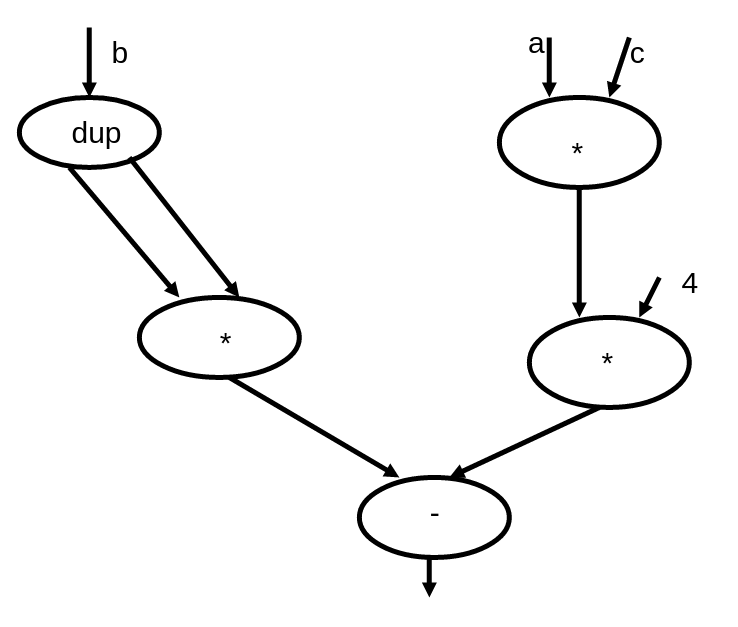
\includegraphics[width=0.5\textwidth]{diagrams/dataflow-prog}
  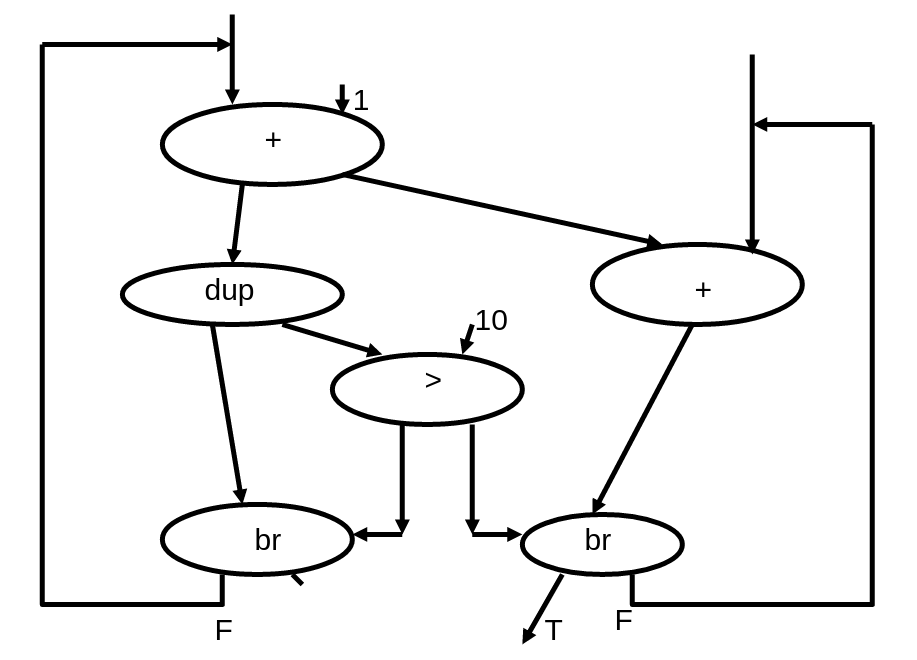
\includegraphics[width=0.5\textwidth]{diagrams/dataflow-loop}
  \caption{A dataflow program and a dataflow program with a loop.}
\end{figure}

To make interesting programs, we need flow control statements that
take a single boolean value and redirect output values
appropriately. Token colouring can be used to make sure different
calls to the same function don't interfere with each other. Graphs can
be self cleaning (ensure that no values remain in the graph once the
function/execution has finished.

The architecture of a dataflow processor is like so:

\begin{figure}[H]
  \centering
  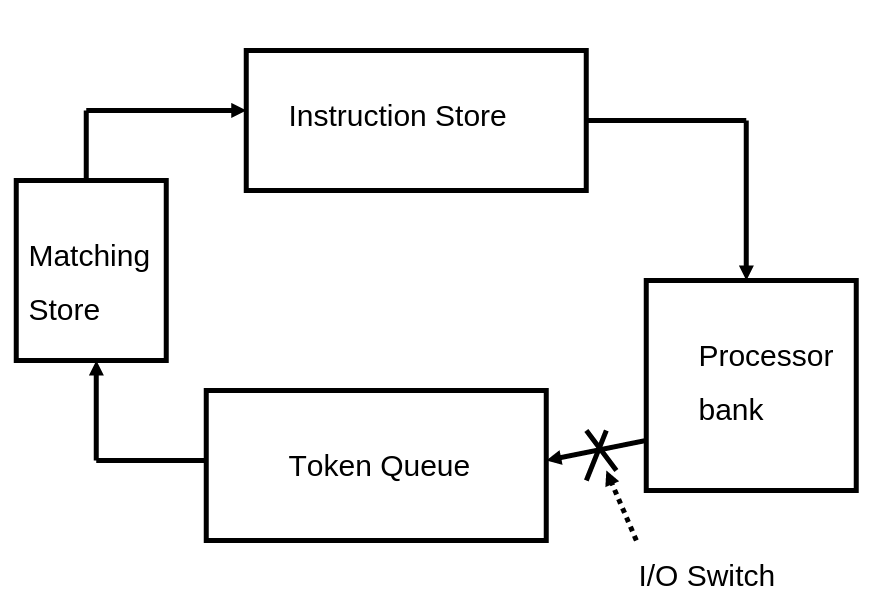
\includegraphics[width=0.5\textwidth]{diagrams/dataflow-arch}
  \caption{The Dataflow Processor Architecture.}
\end{figure}

It contains the following components:

\begin{description}
\item \textbf{Instruction Store}: Holds the coding of the dataflow graph
\item \textbf{Processor Bank}: $n$ processors, all with no state between cycles
\item \textbf{Token Queue}: A buffer to store input data
\item \textbf{Matching Store}: Where tokens with the same colour are marshalled
together to be sent to the same instruction.
\end{description}

Programming for this architecture can be done with assembly code which
is very tedious, or at a higher level language such as with functional
languages. SISAL was developed at Manchester and other institutions as
a programming language that programmers with an imperative background
could use to write programs that could be compiled down to run on a
dataflow processor.

% Bibliography
\bibliography{bib}{}
\bibliographystyle{plain}
